%\documentclass[14pt, a4paper]{report}	%[шрифт, формат]{стиль-book, article, report, proc}. 
\documentclass[14pt, a4paper]{extreport}
\usepackage{ucs}							%хз
\usepackage{cmap}						%решение трабла с крокозябрами в pdf
\usepackage{mathtext}					%отображение кириллицы в формулах
\usepackage[utf8x]{inputenc}				%Включаем поддержку UTF8
\usepackage[T2A]{fontenc}				%Поддержка кириллицы в ЛаТеХ
\usepackage[russian]{babel}				%Включаем пакет для поддержки русского языка
%\DeclareSymbolFont{T2Aletters}{T2A}{cmr}{m}{it}	%Наклоненная кириллица в формулах для latex
%\DeclareSymbolFont{letters}{\encodingdefault}{\rmdefault}{m}{it}					 %для xelatex

%XeTeX packages
%\usepackage[cm-default]{fontspec} % or install lmodern and remove cm-default opt
%\usepackage{xunicode} % some extra unicode support
%\usepackage{xltxtra} % \XeLaTeX macro
%\usepackage{xecyr}
% Setting default fonts
%\setromanfont{Charis SIL}
%\setsansfont{Liberation Sans}
%\setmonofont{Inconsolata}
%\setmainfont{Anonymous Pro} % this allows to use sans-serif as default font  Anonymous Pro

\usepackage{mathtools}
\usepackage{amssymb,amsfonts,amsmath}	%Матпакеты
\newcommand{\argmin}{\arg\!\min}
%
%\begin{align*}
%RQSZ \\
%\mathcal{RQSZ} \\
%\mathfrak{RQSZ} \\
%\mathbb{RQSZ}
%\end{align*}

\usepackage{lipsum}

\usepackage{textcomp}					%Пакет, в котором определен \No под командой \textnumero
\newcommand*{\No}{\textnumero}

\usepackage{wrapfig}
\usepackage{graphicx}
\usepackage{subcaption}
\graphicspath{{pictures/}}
\DeclareGraphicsExtensions{.pdf, .jpg, .png}

\usepackage{indentfirst}

%\pagestyle{headings}

%\usepackage{fancyhdr}					%колонтикулы
%\thispagestyle{fancy}
%\fancyhead{}
%\renewcommand{\headrulewidth}{0 mm}
%\renewcommand{\footrulewidth}{0.15 mm}
%\fancyfoot[L]{test\\}


\footskip = 7pt						%для сносок, команда - \foornote[num]{text}
\renewcommand{\footnoterule}{\vspace{-3pt}\hrule \vspace{2.7pt}}

\usepackage{geometry} %способ ручной установки полей
\geometry{top=2cm} %поле сверху
\geometry{bottom=3cm} %поле снизу
\geometry{left=2cm} %поле справа
\geometry{right=2cm} %поле слева

\usepackage[hidelinks]{hyperref}			%Пакет определяет строки в заголовке как гиперссылки
\addto{\captionsrussian}{\renewcommand*{\contentsname}{Содержание}}
%\usepackage[explicit]{titlesec}
%\titleformat{\section}
%  {\normalfont\normalsize\bfseries\centering}{}{0em}{\MakeUppercase{#1}}

%\usepackage{sectsty}
%\renewcommand{\familydefault}{\rmdefault}

\usepackage{listings}		%Вставка кода

\usepackage{caption}
\captionsetup[table]{singlelinecheck=false}		% Заголовок таблиц слева
\captionsetup{aboveskip=2pt}			%belowskip=6pt 	% Позиционирование заголовка

\ttfamily
%\rmfamily
%\sffamily
%\normalfont
%\renewcommand{\familydefault}{\sfdefault}
%\renewcommand*\sfdefault{pag}
%\allsectionsfont{\centering}
%Serif Fonts
%cmr - Computer Modern Roman (default)
%lmr - Latin Modern Roman
%pbk - Bookman
%bch - Charter
%pnc - New Century Schoolbook
%ppl - Palatino
%ptm - Times
%
%Sans Serif Fonts
%cmss - 	Computer Modern Sans Serif (default)
%lmss - 	Latin Modern Sans Serif
%pag - Avant Garde
%phv - Helvetica
%
%Typewriter Fonts
%cmtt	 - Computer Modern Typewriter (default)
%lmtt	 - Latin Modern
%pcr - Courier

					%\slshape - переключает шрифт на наклонный (вернуть назад \upshape).
					%\bfseries и \mdseries - полужирный.
					%\itshape - курсив.
					%\hspace{1cm} — горизонтальный отступ 1 сантиметр длиной.
					%\noindent — следующий абзац без отступа.
					%\Large — текст большими буквами.
					%\textsc — текст капителью.
					%\textbf — текст жирным шрифтом.
					%\hrulefill - линия вдоль всего документа.
					%\newpage
					%\newline
					%\setcounter{page}{2} - установка счетчика страниц.
					%\tableofcontents - Автоматически генерит содержание.
					%\thispagestyle{empty} - не нумеровать первую страницу.
					%\linebreak - переход на следующую строку.
					%\parindent=2cm - абзацный отступ.
					%\marginpar{abs} - маргиналии (текст на полях)
					
\date{\today}
\title{}
\author{Dema Nikolay}

\usepackage{array,multirow}
\usepackage{cite}


%\addtolength{\parskip}{-1.3cm}
%\setlength{\textfloatsep}{2pt plus 1.0pt minus 2.0pt}
\newcommand{\squeezeup}{\vspace{-4mm}}
\newcommand{\squeezeeup}{\vspace{-2mm}}
\newcommand{\squeezeedown}{\vspace{2mm}}
\newcommand{\squeezeeedown}{\vspace{1mm}}

\newcommand*{\addheight}[2][.5ex]{%
  \raisebox{0pt}[\dimexpr\height+(#1)\relax]{#2}%
}

\linespread{1.2}

\begin{document}
\begin{titlepage}

\begin{center}
\textsc{Санкт-Петербургский национальный исследовательский университет 
                информационных технологий, механики и оптики} \\*
\vspace{0.5cm}
Кафедра Систем управления и информатики \\     

\vspace{0.5cm}
Дисциплина: Динамика робототехнических систем (м.1.3.4-СУиИ)\\     
\end{center}

\vspace{4cm}

%\begin{center}
%\Large Реферат на тему:
%\end{center}

\vspace{0.3cm}

\begin{center}
\large{\textbf{Реферат}}
\end{center}
\begin{center}
\large{\textbf{ВЫВОД УРАВНЕНИЙ ДВИЖЕНИЯ\\ МОБИЛЬНОГО МАНИПУЛЯТОРА}}
\end{center}
\vspace{1cm}



\vspace{4.5cm}

{\small
\begin{flushright}
\parbox{4cm}{\hbox to 3cm{Студент:\hfill} 
			 \hbox to 3cm{Группа:\hfill}
			 \hbox to 3cm{Преподаватель:\hfill}}
\parbox{4cm}{Дема Н.Ю.\\
			 P4135\\
			 Колюбин С. А.}
\end{flushright}}
\vspace{\fill}	

\begin{center}
<<Санкт-Петербург 2017>>
\end{center}

\end{titlepage}
\setcounter{page}{1}
\tableofcontents
\newpage 
%{\parindent=0.2cm \large{\textbf{Задание:}}}\\[0.03cm]		%LARGE\huge\Huge
\ \\
\section*{Введение}
\addcontentsline{toc}{section}{Введение} 
 
На сегодняшний день индустриальное производство, характеризующееся массовостью, а так же алгоритмизацией и формализацией всех процессов, традиционно организуется линейно, посредством ленточных конвейеров и промышленных манипуляторов, которые призваны выполнять различные технологические операции, такие как сварка, сборка, нанесение покрытий распылением, контроль качества и т.д. Такой подход  исключает возможность гибкой реорганизации процесса и остается экономически выгодным лишь при массовом производстве однотипной продукции \cite{Yang}.

Текущее состояние научно-технического прогресса делает возможным преодоление недостатков традиционного подхода. Отказ от жёстких конвейерных решений, позволит значительно снизить затраты на оптимизацию и реорганизацию производственных сценариев, а так же даст толчок к развитию персонализированных производств --- предприятия смогут создавать продукцию, настроенную на нужды индивидуальных заказчиков.

\vspace{\fill}
\begin{figure}[!h]
\centering
\captionsetup{justification=centering}
\renewcommand{\figurename}{Рисунок}
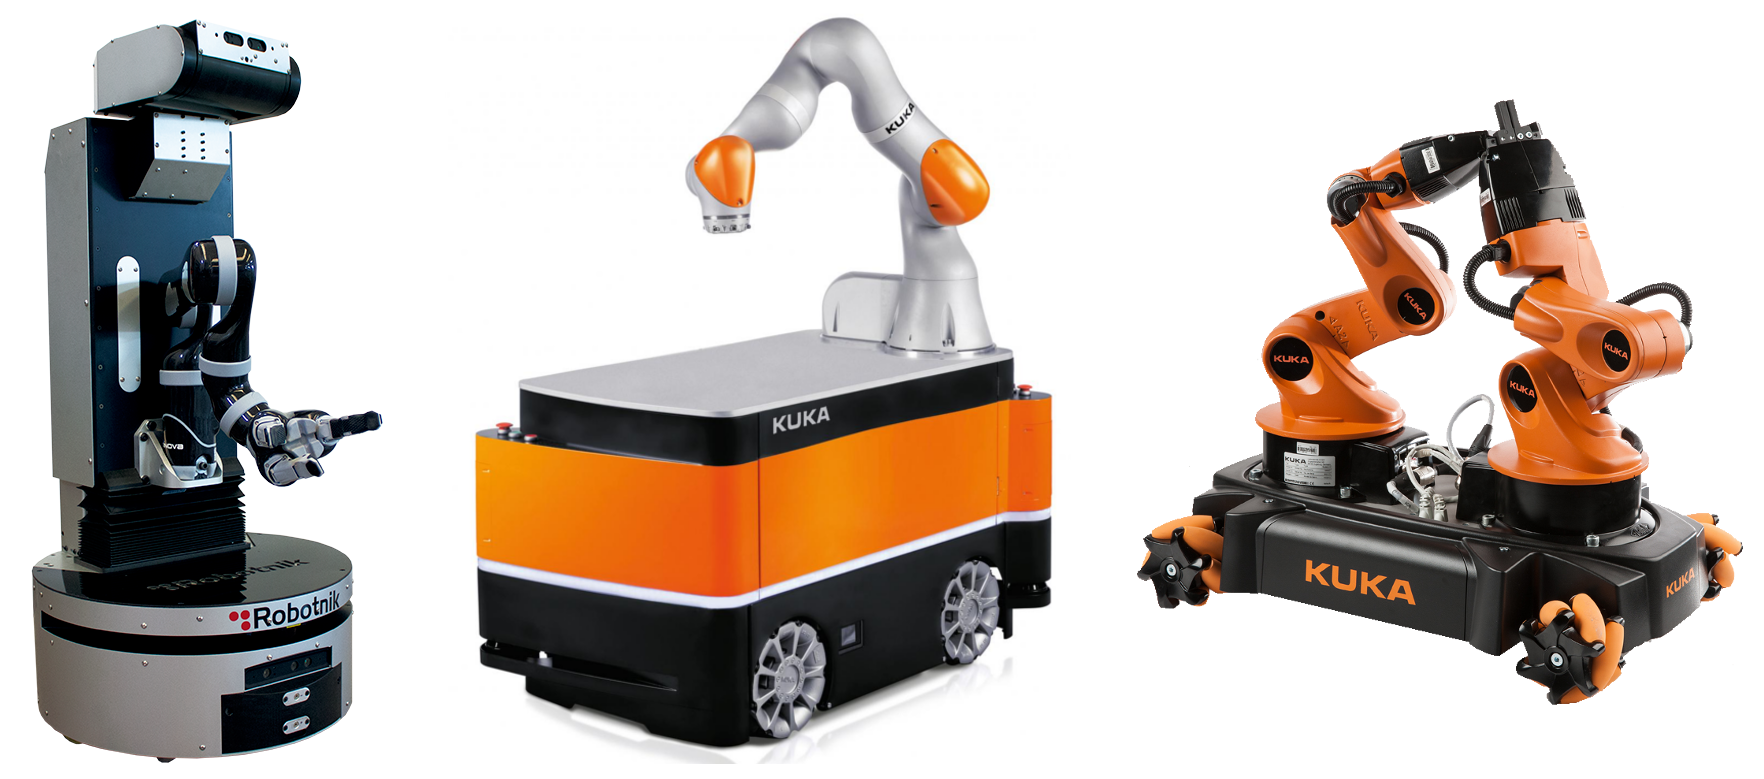
\includegraphics[width=1\textwidth]{mm-.png}	%[width=0.9\textwidth]
\caption{Примеры мобильных манипуляторов на колесной платформе}
\label{pic:1}
\end{figure}
\newpage
\ \\
\vspace{-5mm}
\begin{figure}[!h]
\centering
\captionsetup{justification=centering}
\renewcommand{\figurename}{Рисунок}
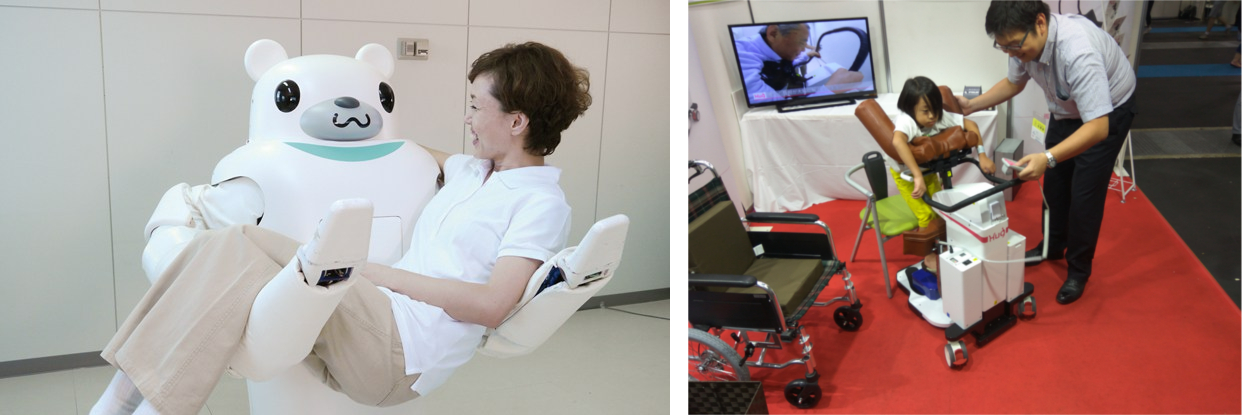
\includegraphics[width=1\textwidth]{med.jpg}	%[width=0.9\textwidth]
\caption{Применение мобильных манипуляторов в медицине для транспортировки пожилых людей и инвалидов}
\label{pic:2}
\end{figure}

Одним из путей организации гибких производств является замещение конвейерных линий мобильными робототехническими платформами, оснащенными манипуляторами (далее --- мобильный манипулятор), что позволит производить транспортировку различных объектов между основными этапами технологического процесса нелинейно и открывает ряд возможностей к его оптимизации в режиме реального времени.

Применение мобильных манипуляторов не ограничивается областью промышленности, примером приложений в области медицины являются роботы помогающие в уходе за инвалидами и пожилыми людьми (Рис. \ref{pic:2}). Мобильные манипуляторы являются чуть ли не единственным доступным на данный момент средством исследования других планет, они так же находят применение в образовании и различных сервисных приложениях, таких как уход по дому, логистика, мерчандайзинг и многих других областях человеческой деятельности \cite{Fantini, Khatib, Stopp, Jones}. 

Мобильные манипуляторы обычно представляют собой мобильную базу с одним или несколькими манипуляторами устанавливаемыми на ней. Таким образом рабочее пространство манипулятора не ограничивается его геометрией. Робот так же имеет различного рода датчики для получения информации об оперативном пространстве. 

Мобильные манипуляторы можно разделить в зависимости от типа мобильной базы следующим образом:
\newpage
\ \\
\vspace{-5mm}
\begin{figure}[!h]
\centering
\captionsetup{justification=centering}
\renewcommand{\figurename}{Рисунок}
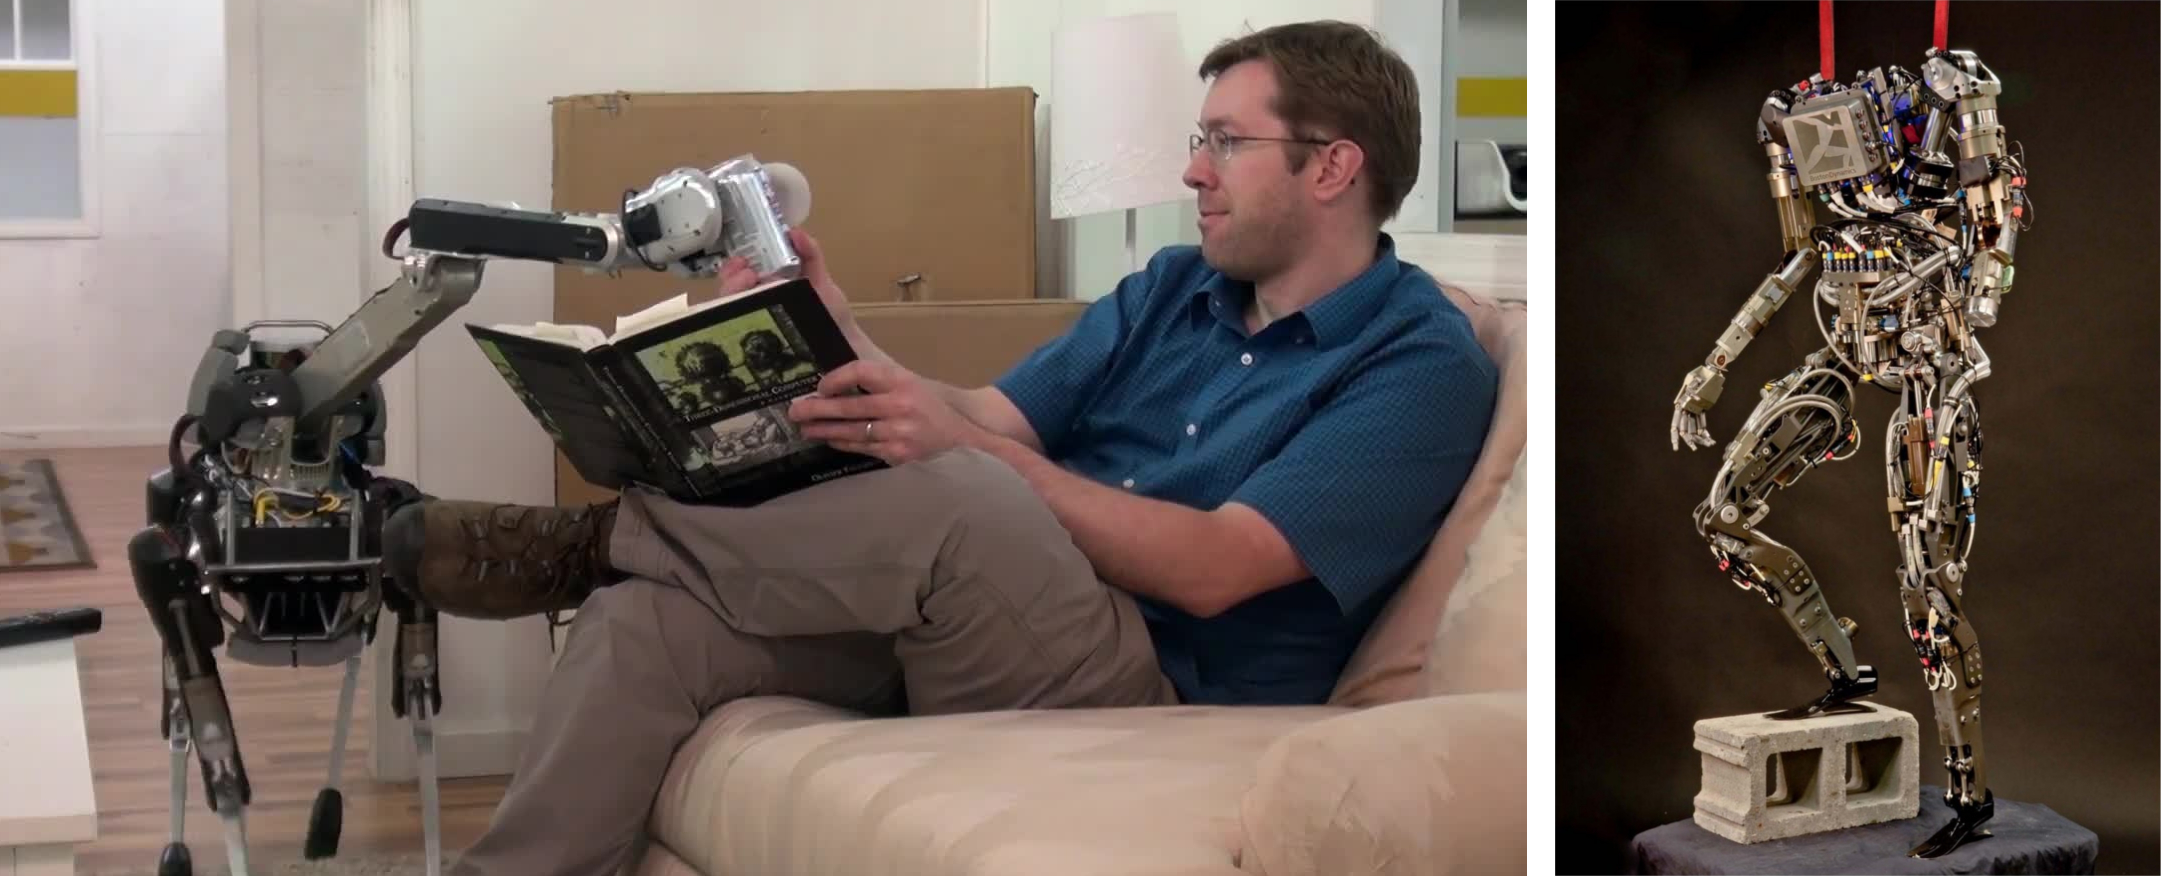
\includegraphics[width=1\textwidth]{darpa.jpg}	%[width=0.9\textwidth]
\caption{Шагающие мобильные манипуляторы Boston Dynamics:\\ SpotMini оснащенный манипулятором с 5-ю степенями свободы и антропоморфный робот Atlas}
\label{pic:3}
\end{figure}
\begin{itemize}
\item Колёсные роботы (см. Рис \ref{pic:1}) --- мобильная база может быть оснащена колесами различного количества и типа (стандартные, поворотные, шведские, всенаправленные, сферические)
\item Гусеничные роботы --- обеспечивают большее сцепление при перемещении по неровным поверхностям относительно баз колесного типа
\item Шагающие роботы (см. Рис \ref{pic:3}) --- для передвижения используются одна (прыгающие роботы) и более ног, имеют ряд преимуществ перед колесными и гусеничными базами. Перемещение робота таким способом представляет собой сложную задачу динамики, а так же требуют более сложного аппаратного и программного обеспечения
\item Летающие роботы (см. Рис \ref{pic:4}) --- новое, активно развивающееся направление в области мобильных манипуляторов \cite{Yang}.
\item Плавающие роботы --- в классе мобильных манипуляторов такие роботы являются преимущественно подводными и служат для исследования и поисково-спасательных операций.
\end{itemize}
\newpage
\begin{figure}[!h]
\centering
\captionsetup{justification=centering}
\renewcommand{\figurename}{Рисунок}
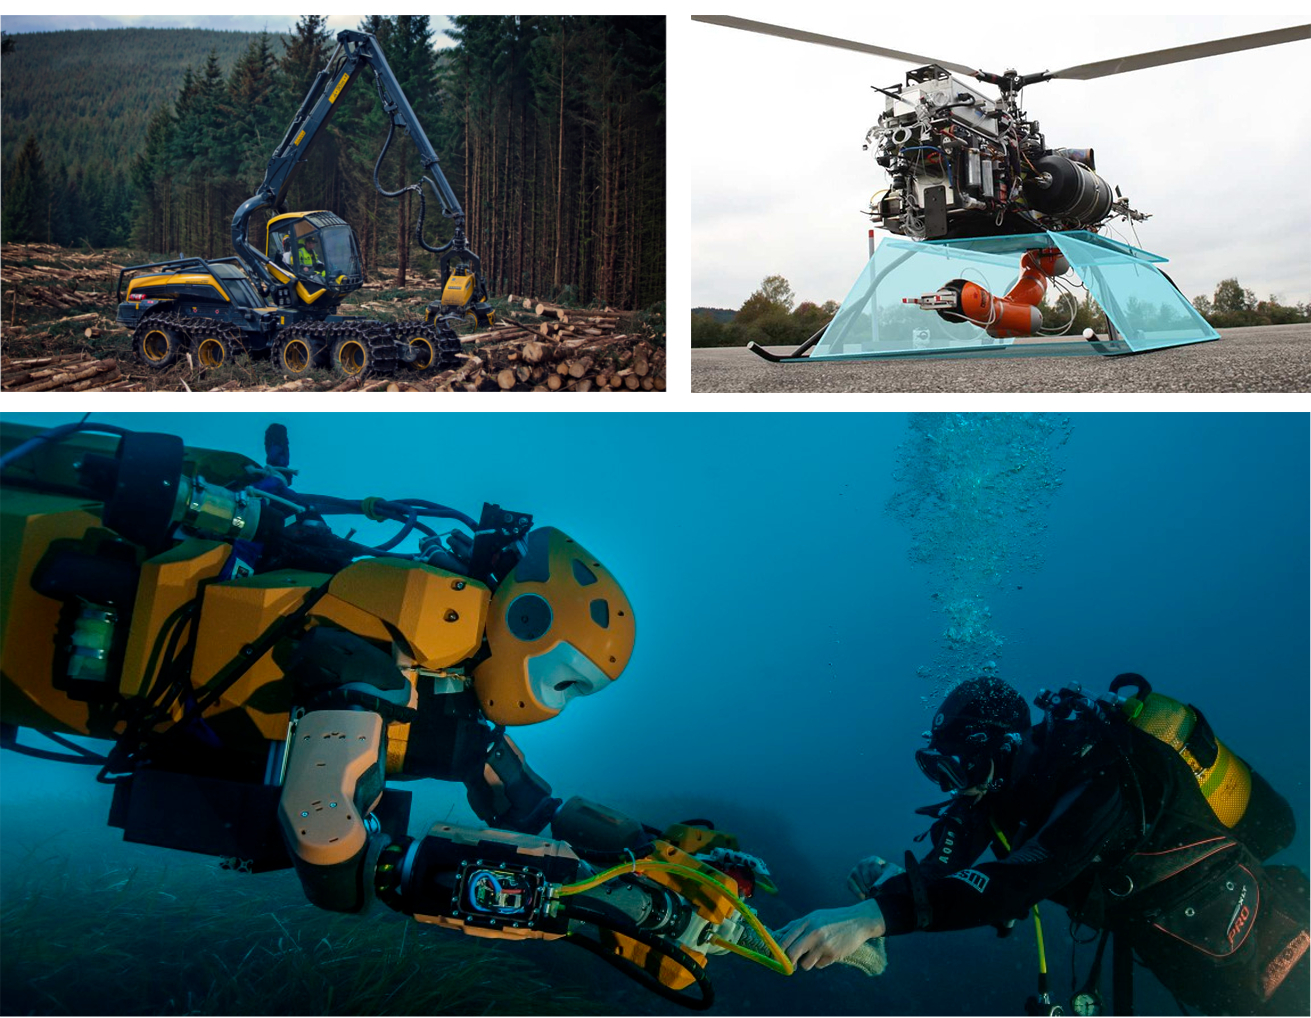
\includegraphics[width=1\textwidth]{big_mm2.jpeg}	%[width=0.9\textwidth]
\caption{Примеры приложений исследуемых систем}
\label{pic:4}
\end{figure}


Сложность математического описания, управления и ряда других задач зависит от типа платформы, а так же возрастает с усложнением структуры робота. Данный реферат ставит своей целью рассмотреть особенности, связанные с получением уравнений движения мобильных манипуляторов имеющих колесную базу, так же, на примере мобильного манипулятора с дифференциальной колесной платформой и манипулятором последовательной кинематики вывести такие уравнения одним из способов, рассматриваемых в следующем разделе.
\newpage

\ \\
\hypertarget{sec:1}{}
\section*{1. \ Обзор существующих решений}
\addcontentsline{toc}{section}{1. Обзор существующих решений} 

Вывод уравнений динамики для мобильных манипуляторов в общем виде является в целом нетривиальной задачей ввиду огромного разнообразия систем такого типа. При выводе уравнений динамики исследуемых систем используются различные законы и формулировки общих уравнений динамики. Среди них можно выделить методы, основанные на уравнениях Эйлера---Лаг­ранжа, Ньютона---Эйлера, Гиббса-Аппеля и Кейна.

Получение уравнений динамики методом Эйлера-Лагранжа отличается простотой и единством подхода, обеспечивает строгое описание состояния системы, и может быть использовано для разработки усовершенствованных законов управления и способов описания самих систем. В меньшей степени такой метод используется для решения прямой и обратной задач динамики ввиду низкой вычислительной эффективности преобразований, таких например как взятие частных производных и матричные преобразования, лежащих в основе данного метода. 

%его уравнений, обусловленной  в основном тем, что для описания кинематической цепи используются матрицы преобразования однородных координат.

Для получения уравнений движения методом Эйлера-Лагранжа в контексте мобильных колесных платформ используют его вариант, включающий в уравнения неопределенные множители Лагранжа для учета неголономных связей \cite{Adamov, Papad, Spyros, Zac}.

Методы, основанные на уравнениях Ньютона---Эйлера обладают большей вычислительной эффективностью, что связанно с их векторным представлением и рекуррентной природой. Пример применения такого метода для рассматриваемых систем, включающих как голономные, так и неголономные связи рассмотрен в \cite{Saha}.

В работе \cite{Korayem} уравнения динамики мобильного манипулятора получены используя формализм Гиббса-Аппеля, где в основе лежит функция "энергии ускорения"\ Гиббса, которая для $i$-го звена системы может быть выражена как:
%\vspace{-1mm}
\begin{equation}
S_i = \frac{m_i a_i^2}{2}  + \frac{\varepsilon_i^T I_i \varepsilon_i}{2}  + 2 (\omega_i \times I_i \omega_i) \varepsilon_i,
\end{equation}
\ \\
\noindent
где $\omega_i, \varepsilon_i, a_i$ --- угловая скорость, угловое и линейное ускорение соответственно, выраженные в начальной системе отсчета, $m_i$ и $I_i$ --- масса и момент инерции для $i$-го звена. Для получения уравнений движения, выраженных относительно обобщенных координат рассчитывается функция Гиббса-Аппеля, определяемая как:

\begin{equation}
\frac{\partial S}{\partial \ddot q_i} = Q_i, (i=1,...,n),
\end{equation}
\noindent
где $S$ --- полная "энергии ускорения"\ Гиббса, определяемая как:
\begin{equation}
S = \sum_{i=1}^n S_i.
\end{equation}

Метод Кейна, приобретающий все большую популярность при получении уравнений динамики \cite{Hussain, Tanner, Ariff}, сочетает в себе положительные стороны методов Ньютона---Эйлера и Эйлера---Лагранжа. 

Метод основан на векторных преобразованиях, что значительно упрощает вычисления по сравнению с методами, в основе которых лежат операции дифференцирования, например Эйлера---Лаг­ранжа и Гиббса-Аппеля. В методе Кейна силы и моменты, не влияющие на динамические уравнения, устраняются в начале расчетов и, следовательно, значительно упрощают расчеты, а вид получаемых уравнений позволяет интерпретировать физический смысл компонент, входящих в уравнения

В работе \cite{Hussain} кратко описана последовательность действий для получения уравнения движения по методу Кейна.
\newpage
\ \\

\section*{2. \ Вывод уравнений движения}
\addcontentsline{toc}{section}{2. Вывод уравнений движения}

Воспользуемся формализмом Эйлера---Лаг­ранжа для вывода уравнений мобильного манипулятора в ввиду его наглядности и простоты интерпретации элементов уравнения по отношению к другим подходам.

При выводе уравнений будем полагать, что система идеальна: отсутствует трение и упругость в сочленениях, отсутствуют проскальзывания при движении мобильной платформы, звенья считаются абсолютно твердыми. Все параметры требуемые для расчетов параметры, такие как массы и моменты инерции звеньев, их геометрия, относительные положения и т.д. известны.

\subsection*{2.1 \ Кинематика мобильных манипуляторов}
\addcontentsline{toc}{subsection}{2.1 Кинематика мобильных манипуляторов}

Как описывалось ранее, мобильный манипулятор состоит из мобильной базы и манипулятора, устанавливаемого на нее. На рисунке \ref{pic:5} изображен пример такой системы, мобильная база которой имеет дифференциальный привод. Обозначим следующие системы координат:\\[2mm]
$O x_w y_w z_w$ --- инерциальная система координат,\\[2mm]
$O x_b y_b z_b$ --- система координат связанная с мобильной базой,\\[2mm]
$O x_m y_m z_m$ --- нулевая система координат манипулятора,\\[2mm]
$O x_e y_e z_e$ --- система координат, связанная с рабочим органом,\\[2mm]
$\psi$ --- угол между векторами $\vec{x}_w$ и $\vec{x}_b$,\\[2mm]
$\upsilon_{j}^{i}$ --- линейная скорость начала $O x_j y_j z_j$ выраженная относительно $O x_i y_i z_i$.\\[2mm]
%$r_{j}^{i}$ --- вектор из начала $O x_j y_j z_j$ в начало $O x_i y_i z_i$,\\[2mm]
\indent
Запишем в векторном виде выражение для определения положения и ориентации рабочего органа манипулятора в инерциальной системе координат как:

\begin{equation}
{^wr_e} = F(q),
\tag{4} \label{eq:4}
\end{equation}
\newpage
\begin{figure}[!h]
\centering
\captionsetup{justification=centering}
\renewcommand{\figurename}{Рисунок}
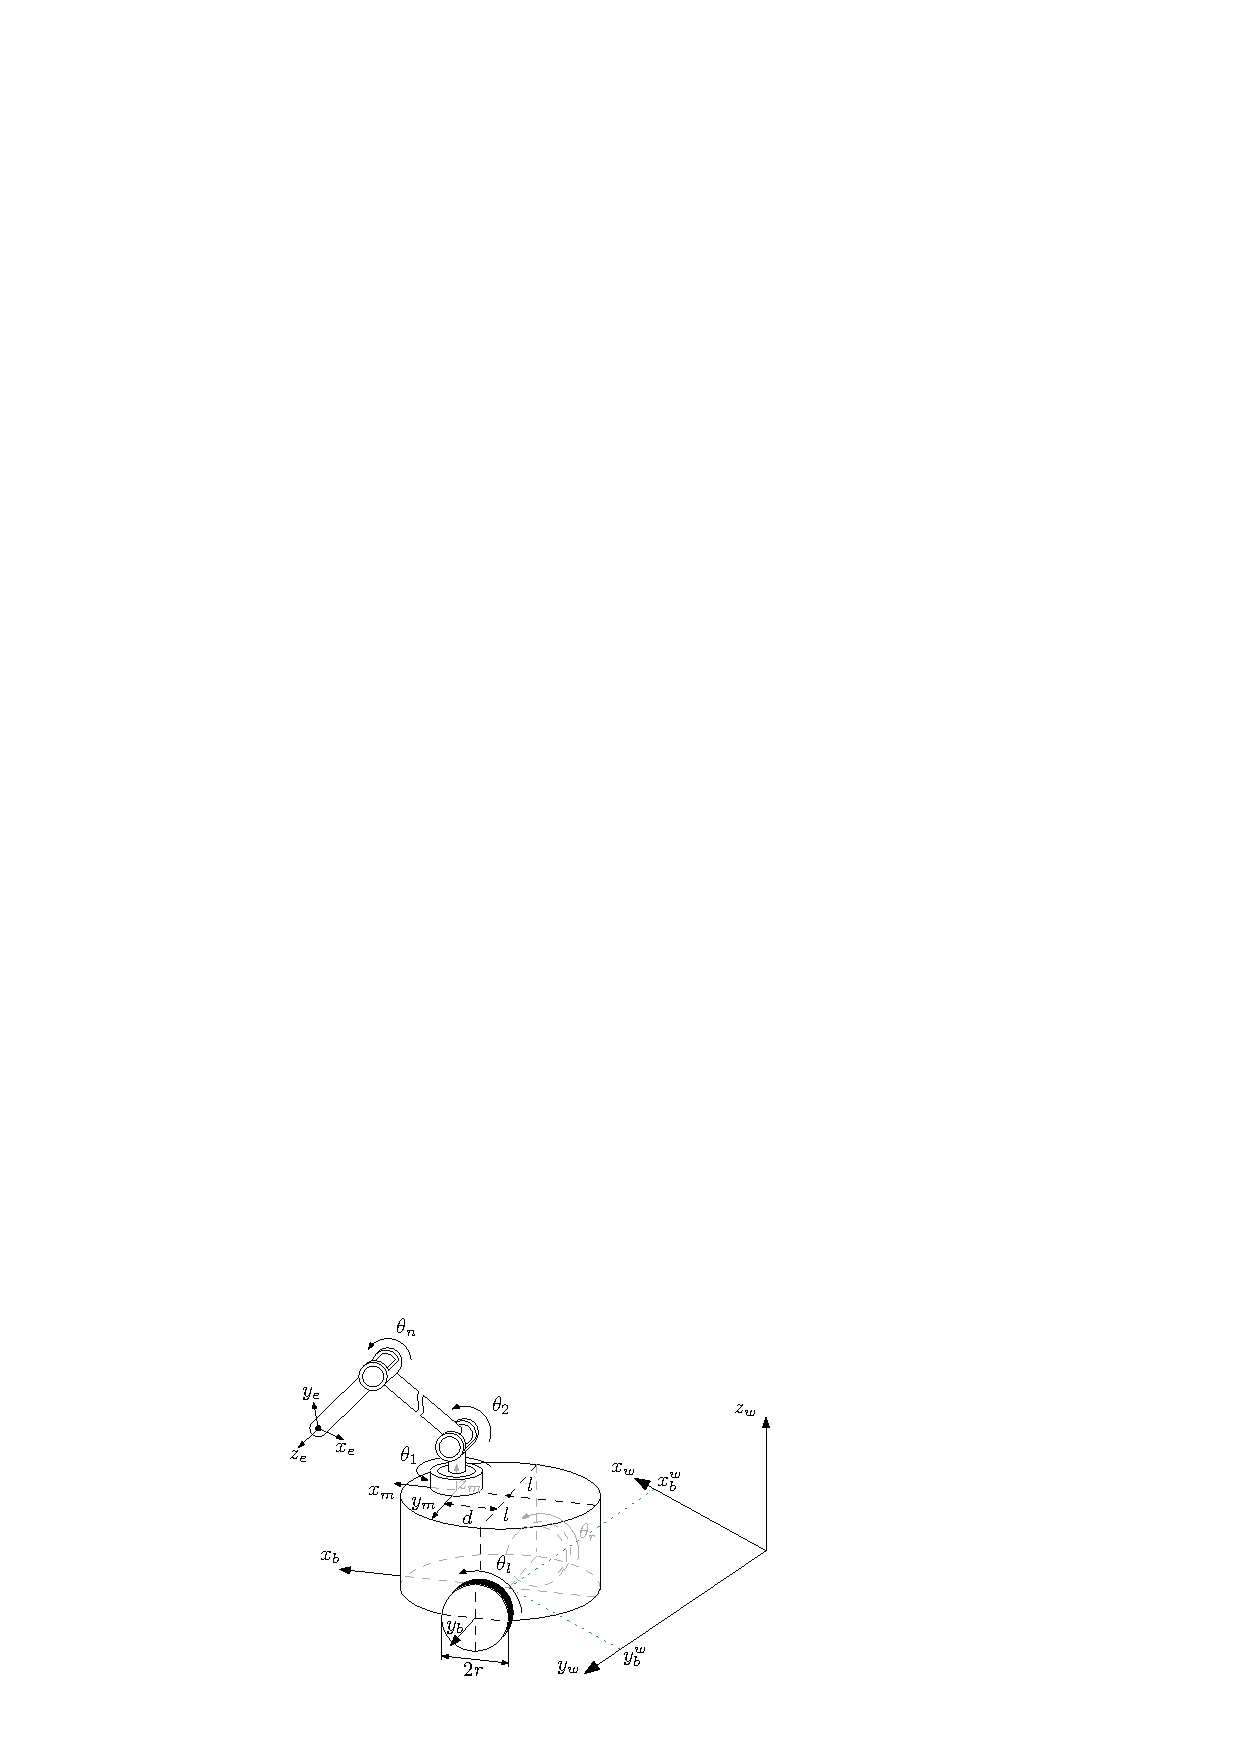
\includegraphics[width=0.88\textwidth]{MM3.pdf}	%[width=0.9\textwidth]
\caption{графическое представление исследуемой системы}
\label{pic:5}
\end{figure}

\noindent
где:\\[3mm]
$q = [q_b^T,q_m^T]^T,$\\[3mm]
$q_b = [x^w_b, y^w_b, \psi]^T$ --- положение базы в инерциальной системе координат,\\[3mm]
$q_m = [q_{m1}, q_{m2}, ..., q_{mn_m}]^T$ --- обобщенные координаты манипулятора.\\[2mm]



Дифференцируя по времени уравнение \ref{eq:4} получим кинематическую модель в обобщенных координатах:

\begin{equation}
{^w\dot{r}_e} = \left(\frac{\partial F}{\partial q_b}\right)\dot{q}_b + \left(\frac{\partial F}{\partial q_m}\right)\dot{q}_m ,
\tag{5} \label{eq:5}
\end{equation}

\noindent
где $\dot{q}_b$ --- определяется исходя из кинематической модели базы и в общем случае выражается как:

\begin{equation}
\dot{q}_b = G(q_b)u_{q_b}, \ \ |u_{q_b}| \leqslant |\dot{q}_b|\!,
\tag{6} \label{eq:6}
\end{equation}
\ \\
\noindent
где $G(q_b)$ --- определяется типом используемой базы, а $u_{q_b} = [\dot{\theta}_r, \dot{\theta}_l]$ --- вход системы в виде скоростей двух управляемых колес.

Рассматриваемая база состоит из двух управляемых колёс и одного пассивного. Движение и ориентирование робота реализуется путем использования двух независимых моторов, передающих моменты на управляемые колеса. Движение базы такого типа ограничивается стационарными неголономными связями, которые в общем виде имеют вид:

\begin{equation}
A(q_b)\dot{q}_b = 0, A \in R^{s\times|q_b|},
\tag{7} \label{eq:7}
\end{equation}

\noindent
где $A(q_b)$ --- прямоугольная матрица, элементы которой являются функциями обобщённых координат, $s$ --- определяется количеством накладываемых на систему неголономных связей.

Для рассматриваемой базы неголономные связи определяются исходя из ее способности двигаться исключительно по нормали к оси управляемых задних колёс, а так же тем условием, что колеса базы двигаются без проскальзывания. Первый факт выражается в следующем уравнении:

\begin{equation}
\dot{x}^w_b\sin(\psi) - \dot{y}^w_b\cos(\psi) = 0.
\tag{8} \label{eq:8}
\end{equation}

Условие движения колес базы без проскальзывания определяется как:

\begin{equation}
\dot{x}^w_b\cos(\psi) + \dot{y}^w_b\sin(\psi) + l\dot{\psi} = r\dot{\theta}_r,
\tag{9} \label{eq:9}
\end{equation}
\begin{equation}
\dot{x}^w_b\cos(\psi) + \dot{y}^w_b\sin(\psi) - l\dot{\psi} = r\dot{\theta}_l,
\tag{10} \label{eq:10}
\end{equation}

Перепишем вектор обобщенных координат базы как $q_b = [x^w_b, y^w_b, \psi, \theta_r, \theta_l]^T$ и сформируем матрицу $A(q_b)$:

\begin{equation}
A(q_b) = 
\begin{bmatrix}
-\sin(\psi) & \cos(\psi) & 0 & 0 & 0 \\[1mm]
\cos(\psi) & \sin(\psi) & l & -r & 0 \\[1mm]
\cos(\psi) & \sin(\psi) & -l & 0 & -r
\end{bmatrix}.
\tag{11} \label{eq:11}
\end{equation}

Тогда матрица $G(q_b)$ из (\ref{eq:6}) может быть сформирована из множества линейно независимых векторов входящих в нуль-пространство матрицы A(q) \cite{Li}, т.е.
\begin{equation}
G(q_b)^T A(q_b)^T = 0
\tag{12} \label{eq:12}
\end{equation}
\newpage

Так же матрица $G(q_b)$ может быть получена исходя из кинематических зависимостей базы, для этого определим линейные скорости управляемых колес как:

\begin{equation}
\upsilon_l^w = \dot{\theta{_l}}r,\ \ \upsilon_r^w = \dot{\theta{_r}}r,
\tag{13} \label{eq:13}
\end{equation}

\noindent
выразим эти величины относительно начала системы координат $O_b$, являющейся средней точкой между колесами платформы:

\begin{equation}
\upsilon_l^w = \upsilon_b^w + l\dot{\psi} ,\ \ \upsilon_r^w = \upsilon_b^w - l\dot{\psi},
\tag{14} \label{eq:14}
\end{equation}

\noindent
складывая и вычитая $\upsilon_l^w$ и $\upsilon_l^w$ получим:

\begin{equation}
\upsilon_b^w = \frac{1}{2}(\upsilon_r^w + \upsilon_l^w),\ \ \dot{\psi} = \frac{1}{2l}(\upsilon_r^w - \upsilon_l^w).
\tag{15} \label{eq:15}
\end{equation}

Учитывая:

\begin{equation}
\dot{x}_b^w = \upsilon_b^w\cos(\psi) ,\ \ \dot{y}_b^w = \upsilon_b^w\sin(\psi),
\tag{16} \label{eq:16}
\end{equation}

\noindent
запишем кинетическую модель базы:

\begin{equation}
\dot{x}_b^w = \frac{r}{2}(\dot{\theta}_r\cos(\psi) + \dot{\theta}_l\cos(\psi)),
\tag{17} \label{eq:17}
\end{equation}
\begin{equation}
\dot{y}_b^w = \frac{r}{2}(\dot{\theta}_r\sin(\psi) + \dot{\theta}_l\sin(\psi)),
\tag{18} \label{eq:18}
\end{equation}
\begin{equation}
\dot{\psi} = \frac{r}{2l}(\dot{\theta}_r - \dot{\theta}_l).
\tag{19} \label{eq:19}
\end{equation}

Тогда полная кинематическая модель базы с учетом смещения точки крепления манипулятора относительно начала системы координат $O_b$ может быть записана в форме (\ref{eq:6}):

\begin{equation}
\begin{bmatrix}
\dot{x}^w_b\\[1mm] \dot{y}^w_b\\[1mm] \dot{\psi}\\[1mm] \dot{\theta}_r\\[1mm] \dot{\theta}_l
\end{bmatrix} = 
\begin{bmatrix}
\frac{r}{2}(\cos(\psi) - dl\sin(\psi)) & \frac{r}{2}(\cos(\psi) + dl\sin(\psi))\\[1mm]
\frac{r}{2}(\sin(\psi) + dl\cos(\psi)) & \frac{r}{2}(\sin(\psi) - dl\cos(\psi))\\[1mm]
\frac{r}{2l} & -\frac{r}{2l}\\[1mm]
1 & 0\\[1mm]
0 & 1\\[1mm]
\end{bmatrix}
\begin{bmatrix}
\dot{\theta}_r\\[1mm] \dot{\theta}_l
\end{bmatrix}.
\tag{20} \label{eq:20}
\end{equation}
\newpage

Стоит заметить, что при записи уравнений неголономных связей могла быть допущена ошибка относительно их действительного количества. В работе \cite{Li} рассматривается подход к определению количества голономных и не голономных связей основываясь свойстве инволютивности распределения, строящегося как совокупность всех линейных комбинаций векторов матрицы $G(q_b)$. Используя такой подход можно определить наличие одной голономной и двух неголономных связей в рассматриваемой системе.

Вычитая (\ref{eq:9}) и (\ref{eq:10}) определим голономную связь:

\begin{equation}
\dot{\psi} = \frac{r}{2l}(\dot{\theta}_r - \dot{\theta}_l)
\tag{21} \label{eq:21}
\end{equation}

\noindent
что эквивалентно соответствующей компоненте в (\ref{eq:20}).Интегрируя уравнение (\ref{eq:21}) и выбирая следующие начальные условия:

\[
\psi(0) = 0,\ \ \theta_r(0) = 0,\ \ \theta_l(0) = 0,
\]

\noindent
получим уравнение

\begin{equation}
\psi = \frac{r}{2l}(\theta_r - \theta_l),
\tag{22} \label{eq:22}
\end{equation}

\noindent
которое представляет собой уравнение голономной связи. Таким образом $\psi$ может быть устранена из вектора обобщённых координат.

Складывая и выражая соответствующим образом (\ref{eq:9}) и (\ref{eq:10}) получим конечные выражения для неголономных связей:

\begin{equation}
\dot{x}^w_b\sin(\psi) - \dot{y}^w_b\cos(\psi) = 0,
\tag{23} \label{eq:23}
\end{equation}
\begin{equation}
\dot{x}^w_b\cos(\psi) + \dot{y}^w_b\sin(\psi) = \frac{r}{2}(\dot{\theta}_r + \dot{\theta}_l)
\tag{24} \label{eq:24}
\end{equation}

Из приведенных выше выражений ясно, что $\psi$ не является независимой переменной и однозначно определяется выражением (\ref{eq:22}). Приняв новый вектор обобщенных координат базы в виде:

\begin{equation}
q_b = 
\begin{bmatrix}
x^w_b\\[1mm] y^w_b\\[1mm] \theta_r\\[1mm] \theta_l
\end{bmatrix}
\tag{25} \label{eq:25}
\end{equation}

\noindent
определим новую матрицу $A(q_b)$ в соответствии с выражениями (\ref{eq:23}) и (\ref{eq:24}):

\begin{equation}
A(q_b) = 
\begin{bmatrix}
-\sin(\psi) & \cos(\psi) & 0 & 0\\[1mm]
\cos(\psi) & \sin(\psi) & -\frac{r}{2} & -\frac{r}{2}\\[1mm]
\end{bmatrix}.
\tag{26} \label{eq:26}
\end{equation}

Для учета проскальзывания колес кинематическую модель может быть дополнена компонентами $w_r$ и $w_l$ для обозначения продольного смещения правого и левого колес соответственно и компонентами $z_r$ и  $z_l$ соответствующим смещению в поперечном направлении. Таким образом, перепишем вектор $q_b$ как:

\begin{equation}
q_b = 
\begin{bmatrix}
x^w_b\\[1mm] y^w_b\\[1mm] \psi\\[1mm] w_r\\[1mm] w_l\\[1mm] z_r\\[1mm] z_l
\end{bmatrix}
\tag{27} \label{eq:27}
\end{equation}

Перепишем выражения для кинематики в соответствии с учетом новых компонент:

\begin{equation}
\upsilon_l^w = \dot{\theta{_l}}r - w_l = \dot{x}_b^w\cos(\psi) + \dot{y}_b^w\sin(\psi) - l\dot{\psi},
\tag{28} \label{eq:28}
\end{equation}

\begin{equation}
\upsilon_r^w = \dot{\theta{_r}}r - w_r = \dot{x}_b^w\cos(\psi) + \dot{y}_b^w\sin(\psi) + l\dot{\psi},
\tag{29} \label{eq:29}
\end{equation}

\begin{equation}
-\dot{x}^w_b\sin(\psi) + \dot{y}^w_b\cos(\psi) = z_r = z_l.
\tag{30} \label{eq:30}
\end{equation}

Тогда, формируя вектор обобщенных координат, как:

\begin{equation}
q_b = 
\begin{bmatrix}
x^w_b& y^w_b& \psi& z_r& z_l& \upsilon_r^w& \upsilon_l^w& \theta_r& \theta_l
\end{bmatrix},
\tag{31} \label{eq:31}
\end{equation}
\vspace{2mm}

\noindent
Матрица $A(q_b)$ приобретет следующий вид:
\newpage
\
\begin{equation}
A(q_b) = 
\begin{bmatrix}
\cos(\psi)  & \sin(\psi) &  l &  0 &  0 & -1 &  0 & 0 & 0\\[1mm]
\cos(\psi)  & \sin(\psi) & -l &  0 &  0 &  0 & -1 & 0 & 0\\[1mm]
-\sin(\psi) & \cos(\psi) &  0 & -1 &  0 &  0 &  0 & 0 & 0\\[1mm]
-\sin(\psi) & \cos(\psi) &  0 &  0 & -1 &  0 &  0 & 0 & 0
\end{bmatrix},
\tag{32} \label{eq:32}
\end{equation}
\ \\
\noindent
где соответствующая ей матрица $G(q_b)$:

\begin{equation}
G(q_b) = 
\begin{bmatrix}
-\sin(\psi)  & \dfrac{1}{2}\cos(\psi) &  \dfrac{1}{2}\sin(\psi) &  0 &  0 \\[3mm]
\cos(\psi)   & \dfrac{1}{2}\cos(\psi) &  \dfrac{1}{2}\sin(\psi) &  0 &  0 \\[3mm]
0 & \dfrac{1}{2l} &  -\dfrac{1}{2l} & 0 &  0\\[2mm]
1 & 0 &  0 &  0 & 0\\[1mm]
1 & 0 &  0 &  0 & 0\\[1mm]
0 & 1 &  0 &  0 & 0\\[1mm]
0 & 0 &  1 &  0 & 0\\[1mm]
0 & 0 &  0 &  1 & 0\\[1mm]
0 & 0 &  0 &  0 & 1
\end{bmatrix},
\tag{33} \label{eq:33}
\end{equation}
\ \\

\noindent
где:

\begin{equation}
u_{q_b} = 
\begin{bmatrix}
\dot{z}_l \\[1mm] \dot{\upsilon}_r^w \\[1mm] \dot{\upsilon}_l^w \\[1mm] \dot{\theta}_r \\[1mm] \dot{\theta}_l
\end{bmatrix}, \ \ (\text{учитывая то, что } z_r = z_l)
\tag{34} \label{eq:34}
\end{equation}
\ 

Частой практикой является исключение из рассмотрения компонент продольного проскальзывания, так как на малых скоростях их значения малы и компенсируются дополнительным сенсорным оснащением робота. 

Описанные выше компоненты обычно неизвестны и неизмеримы, что является одной из основных проблем навигации мобильных платформ.
\newpage

Так же, все большую популярность приобретают колесные всенаправленные платформы, движение которых в плоскости не ограничивается неголономными связями. Это возможно благодаря особой конструкции колес, включающей в себя дополнительные ролики, монтируемые к колесу \cite{Muir}. Ось вращения роликов смещается относительно оси вращения самого колеса на некоторый угол, что и позволяет базе свободно перемещаться в плоскости движения.

Рассмотрим кинематику такой платформы на примере представленной на рисунке \ref{pic:6} базы, имеющей 4 шведских колеса. Обозначим 4 системы координат $O_{wi}$, связанных соответственно с i-ми колесами. Каждое колесо характеризуется вектором угловых скоростей $\dot{q}_i$ и имеет три компоненты:\\[3mm]
$\dot{q}_{ix}$ --- угловая скорость вращения колеса вокруг вала,\\[3mm]
$\dot{q}_{iy}$ --- угловая скорость вращения ролика, контактирующего с поверхностью,\\[3mm]
$\dot{q}_{iz}$ --- угловая скорость вращения колеса вокруг оси, проходящей через точку контакта с поверхностью и перпендикулярной ей.\\[3mm]

Тогда соответствующий вектор скорости $v_{wi} = [\dot{x}_{wi}, \dot{y}_{wi}, \dot{\psi}_{wi}]^T$, выраженный в $O_{wi}$, определяется как:

\begin{equation}
\begin{bmatrix}
\dot{x}_{wi}\\[1mm] \dot{y}_{wi}\\[1mm] \dot{\psi}_{wi}
\end{bmatrix} = 
\begin{bmatrix}
0 & r_i\sin(\alpha_i) & 0\\[1mm]
R_i & -r_i\cos(\alpha_i) & 0\\[1mm]
0 & 0 & 1
\end{bmatrix}
\begin{bmatrix}
\dot{q}_{ix}\\[1mm] \dot{q}_{iy}\\[1mm] \dot{q}_{iz}
\end{bmatrix}\!,
\tag{35} \label{eq:35}
\end{equation}
\ \\

\noindent
где для $i=1..4$ $R_i$ --- радиус колеса, $r_i$ --- радиус ролика и $\alpha_i$ --- угла поворота ролика относительно вала. Скорость базы $v_{b} = [\dot{x}_b, \dot{y}_b, \dot{\psi}_b]^T$ в системе координат центра масс $O_b$ может быть получена как:

\newpage
\begin{figure}[!h]
\centering
\captionsetup{justification=centering}
\renewcommand{\figurename}{Рисунок}
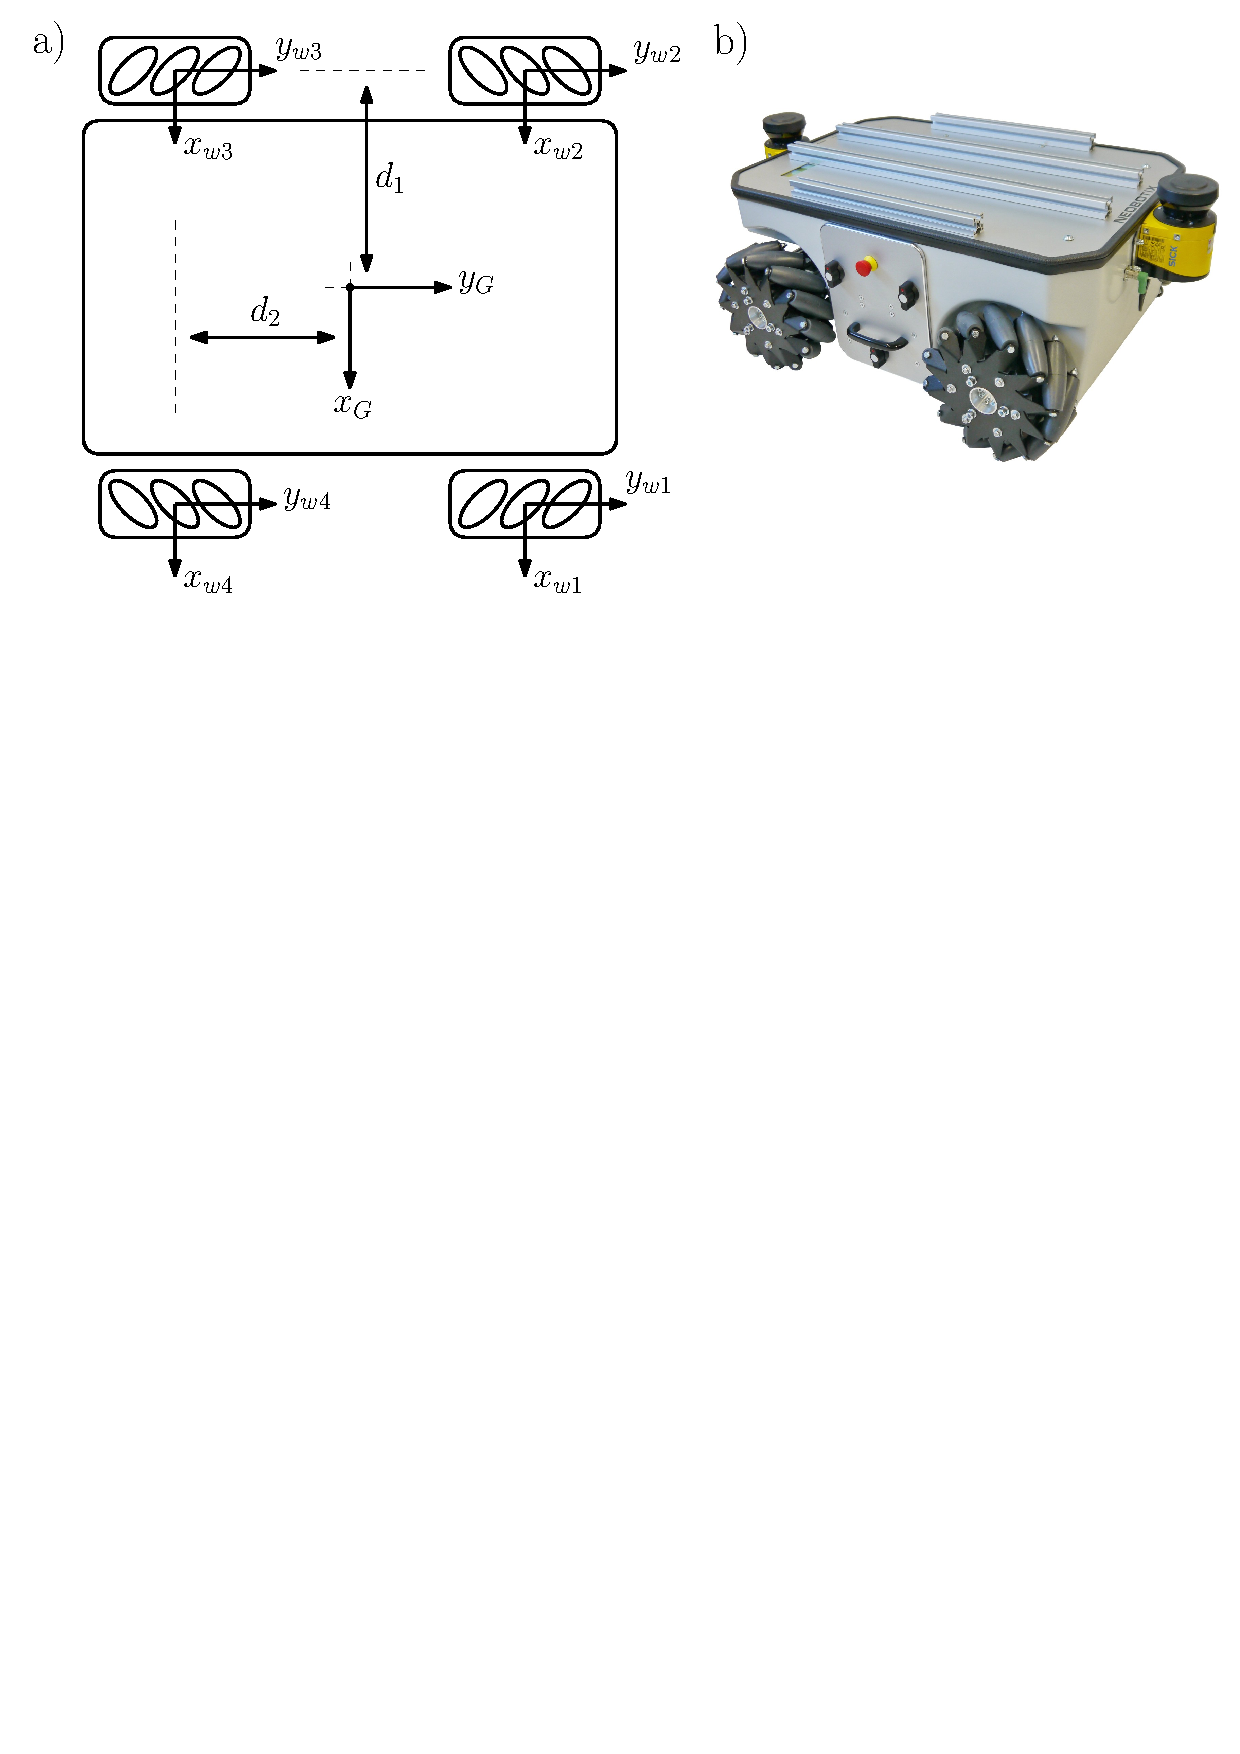
\includegraphics[width=1\textwidth]{omnib.pdf}	%[width=0.9\textwidth]
\caption{Четырехколесная платформа с шведскими колесами: кинематическая схема (а) и пример такой платформы (b)}
\label{pic:6}
\end{figure}

\begin{equation}
v_{b} = 
\begin{bmatrix}
\dot{x}_b\\[1mm] \dot{y}_b\\[1mm] \dot{\psi}_b
\end{bmatrix} = 
\begin{bmatrix}
\cos(\phi_{wi}^b) & -\sin(\phi_{wi}^b) & d_{wiy}^b\\[1mm]
\sin(\phi_{wi}^b) & \cos(\phi_{wi}^b) & -d_{wix}^b\\[1mm]
0 & 0 & 1
\end{bmatrix}
\begin{bmatrix}
\dot{x}_{wi}\\[1mm] \dot{y}_{wi}\\[1mm] \dot{\psi}_{wi}
\end{bmatrix}\!,
\tag{36} \label{eq:36}
\end{equation}

\noindent
где $\phi_{wi}^b$ --- обозначает угол поворота из $O_b$ в $O_{wi}$, а $d_{wiy}^b$ и $d_{wix}^b$ ---соответствующие координаты начала координат $O_{wi}$ в системе координат $O_b$. Подставляя (\ref{eq:35}) в (\ref{eq:36}) получим:

\begin{equation}
v_{b} = J_i v_{wi},
\tag{37} \label{eq:37}
\end{equation}

\noindent
где $J_i$ --- является квадратным и обратимым якобианом i-го колеса и выражается как:

\begin{equation}
J_i = 
\begin{bmatrix}
-R_i\sin(\phi_{wi}^b) & r_i\sin(\phi_{wi}^b + \alpha_i) & d_{wiy}^b\\[1mm]
R_i\cos(\phi_{wi}^b) & -r_i\cos(\phi_{wi}^b + \alpha_i) & -d_{wix}^b\\[1mm]
0 & 0 & 1
\end{bmatrix}\!.
\tag{38} \label{eq:38}
\end{equation}

Положем, что колеса идентичны и перепишем их параметры как:

\[
R_i = R,\ \ r_i = r,\ \ \phi_{wi}^b = 0,
\]
\newpage
\[
d_{wix}^b = d_1,\ \ d_{wiy}^b = d_2,
\]
\[
\alpha_1 = \alpha_3 = 45^{\circ},\ \ \alpha_2 = \alpha_4 = -45^{\circ}.
\]

Тогда соответствующие якобианы можно определить, как:

\[
\begin{gathered} 
J_1 =
\begin{bmatrix}
0 & -r\sqrt{2}/2 & d_2\\[1mm]
R & -r\sqrt{2}/2 & d_1\\[1mm]
0 & 0 & 1
\end{bmatrix}\!\!,\ \ \ 
J_2 =
\begin{bmatrix}
0 & r\sqrt{2}/2 & d_2\\[1mm]
R & -r\sqrt{2}/2 & -d_1\\[1mm]
0 & 0 & 1
\end{bmatrix}\!\!,\\
J_3 =
\begin{bmatrix}
0 & -r\sqrt{2}/2 & -d_2\\[1mm]
R & -r\sqrt{2}/2 & -d_1\\[1mm]
0 & 0 & 1
\end{bmatrix}\!\!,\ \ \ 
J_4 =
\begin{bmatrix}
0 & r\sqrt{2}/2 & -d_2\\[1mm]
R & -r\sqrt{2}/2 & d_1\\[1mm]
0 & 0 & 1
\end{bmatrix}\!\!.
		\tag{39} \label{eq:39}
\end{gathered}
\]

Робот приводится в движение посредством одновременного вращения колес вокруг их валов. Таким образом, определяя обратные якобианы и учитывая при задании скорости только соответствующие компоненты $\dot{q}_{ix}$ получим \cite{Hamid}:

\begin{equation}
\begin{bmatrix}
\dot{x}_b\\[1mm] \dot{y}_b\\[1mm] \dot{\psi}_b
\end{bmatrix} = 
\frac{R}{4}
\begin{bmatrix}
-1 & 1 & -1 & 1\\[1mm]
1 & 1 & 1 & 1\\[1mm]
\dfrac{1}{d_1+d_2} & \dfrac{-1}{d_1+d_2} & \dfrac{-1}{d_1+d_2} & \dfrac{1}{d_1+d_2}
\end{bmatrix}
\begin{bmatrix}
\dot{x}_{w1}\\[1mm] \dot{x}_{w2}\\[1mm] \dot{x}_{w3}\\[1mm] \dot{x}_{w4}\\[1mm]
\end{bmatrix}\!,
\tag{40} \label{eq:40}
\end{equation}

\begin{equation}
\begin{bmatrix}
\dot{x}_{w1}\\[1mm] \dot{x}_{w2}\\[1mm] \dot{x}_{w3}\\[1mm] \dot{x}_{w4}\\[1mm]
\end{bmatrix} = 
\frac{4}{R}
\begin{bmatrix}
-1 & 1 & d_1+d_2\\[1mm]
1 & 1 & -(d_1+d_2)\\[1mm]
-1 & 1 & -(d_1+d_2)\\[1mm]
1 & 1 & d_1+d_2
\end{bmatrix}
\begin{bmatrix}
\dot{x}_b\\[1mm] \dot{y}_b\\[1mm] \dot{\psi}_b
\end{bmatrix}\!.
\tag{41} \label{eq:41}
\end{equation}

Тогда вектор скорости робота в глобальной системе координат $v = [\dot{x}, \dot{y}, \dot{\psi}]^T$ можно определить как:

\begin{equation}
\begin{bmatrix}
\dot{x}\\[1mm] \dot{y}\\[1mm] \dot{\psi}
\end{bmatrix}
= 
\begin{bmatrix}
\cos(\psi) & -\sin(\psi) & 0\\[1mm]
\sin(\psi) & \cos(\psi) & 0\\[1mm]
0 & 0 & 1
\end{bmatrix}
\begin{bmatrix}
\dot{x}_b\\[1mm] \dot{y}_b\\[1mm] \dot{\psi}_b
\end{bmatrix}\!.
\tag{42} \label{eq:42}
\end{equation}
\newpage
\begin{figure}[!h]
\centering
\captionsetup{justification=centering}
\renewcommand{\figurename}{Рисунок}
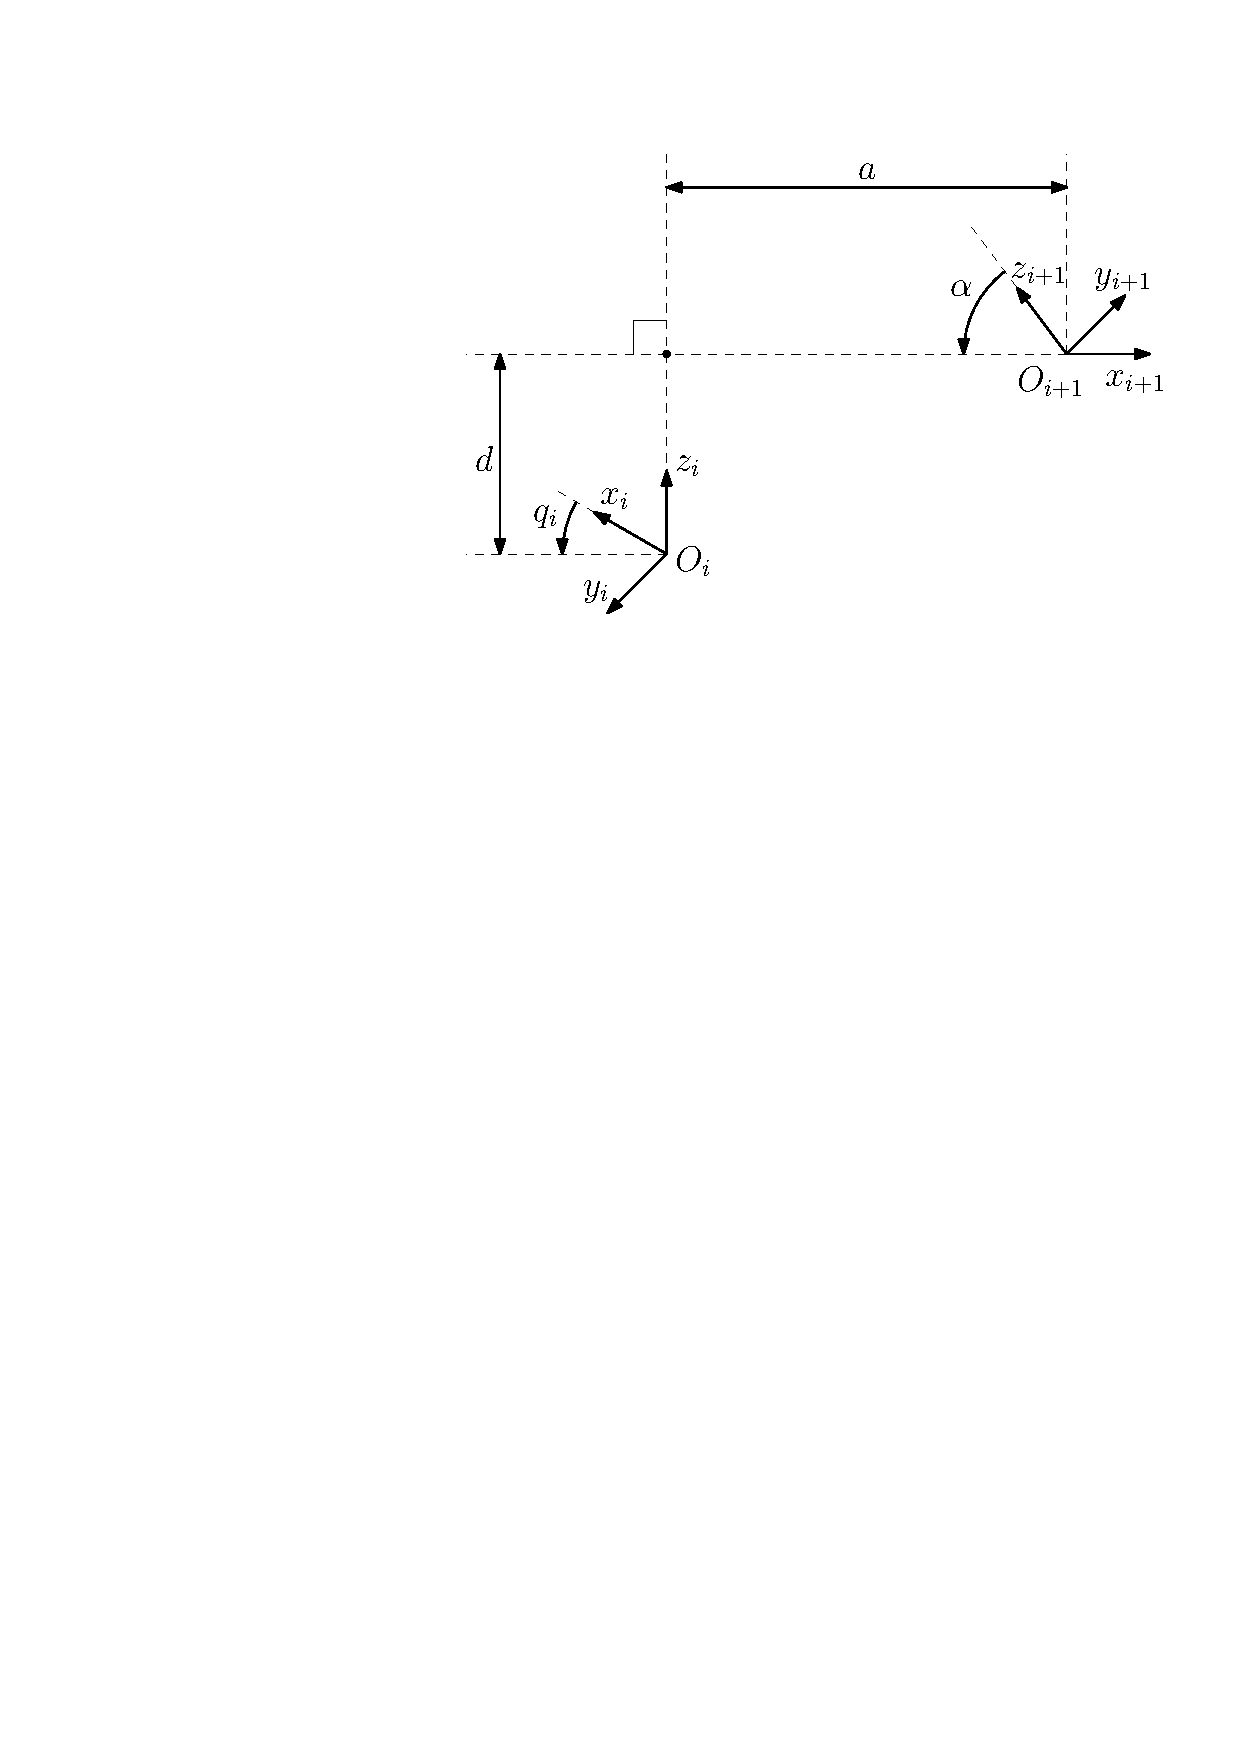
\includegraphics[width=0.82\textwidth]{DH.pdf}	%[width=0.9\textwidth]
\caption{Пример назначения параметров Денавита-Хартенберга}
\label{pic:7}
\end{figure}

Описание кинематики манипулятора обычно состоит из назначения систем координат, положение которых однозначно определяет конфигурацию манипулятора. Для выбора систем координат широко используется метод Денавита --- Хартенберга, который позволяет сократить количество координат, однозначно определяющих соответствующую систему координат в пространстве до 4 \cite{Borisov}. Пример такого назначения систем координат представлен на рисунке \ref{pic:7}. 

После выбора системы координат следуя методу Денавита --- Хартенберга посредством матрицы однородных преобразований:
\[
^{i-1}H_i =
	\begin{bmatrix}
		\cos(q_{mi}) & 	-\sin(q_{mi})\cos(\alpha_i) & 	\sin(q_{mi})\sin(\alpha_i)	&	a_i\cos(q_{mi})\\
		\sin(q_{mi}) & 	\cos(q_{mi})\cos(\alpha_i) &	-\cos(q_{mi})\sin(\alpha_i) &	a_i\sin(q_{mi})\\
		0				&	\sin(\alpha_i) 						&	\cos(\alpha_i)					& 	d_i\\
		0				&	0									&	0								&	1
	\end{bmatrix} \tag{43} \label{eq:43}
\]

\noindent
задают линейное смещение и пространственную ориентацию одной системы относительно другой. Итоговую матрицу, связывающую все системы координат можно получить последовательным перемножением:
\begin{equation}
^{0}H_n(q_{m}) = \prod_{i=1}^{n} \left(^{i-1}H_i\right).
\tag{44} \label{eq:44}
\end{equation}
\newpage

Таким образом, для заданных значений обобщенных координат $q_{m}$  посредством (\ref{eq:44}) можно определить координаты системы, связанной с рабочим органом манипулятора (прямая задача кинематики):
\begin{equation}
^mr_e = {^0H}_n(q_{m})\mathbf{O},
\tag{45} \label{eq:45}
\end{equation}
\vspace{-2mm}
\noindent
где $\mathbf{O}$ --- нулевой вектор размерности $(n_m\times 1)$. 

Обратная же задача кинематики, то есть определение значений обобщенных координат для заданной системы координат, связанной с рабочим органом, в общем случае не имеет явного решения. Для манипуляторов избыточной кинематики или тех случаев, когда манипулятор находится в, так называемом, сингулярном или околосингулярном состоянии, при решении обратной задачи кинематики используют эвристические подходы. Например в работе \cite{Buss} предлагается метод, основанный на сингулярном разложении якобиана, в работах \cite{Ben, Andreas} предлагаются итеративные алгоритмы, основанные на геометрии и кинематических ограничениях манипулятора.

Для манипулятора последовательной кинематики якобиан, связывающий обобщенные скорости с угловыми и линейными скоростями рабочего органа, можно получить как:
\begin{equation}
J(q_m) = 
\begin{bmatrix}
J_1 & J_2 & ... & J_{n_m}
\end{bmatrix},
\tag{46} \label{eq:46}
\end{equation}

\noindent
где $J_i$ --- составляющая якобиана для i-го сочленения манипулятора, для вращательного сочленения определяется как:
\begin{equation}
J_i = 
\begin{bmatrix}
z^0_{i-1} \times (p^0_{n_m} - p^0_{i-1})\\[1mm]
z^0_{i-1}
\end{bmatrix},
\tag{47} \label{eq:47}
\end{equation}

\noindent
где соответствующие величины в общем виде обозначаются как:\\[2mm]
$p^i_j$ --- вектор из начала $Ox_iy_i z_i$ в начало $Ox_i y_i z_i$.\\[2mm]
$z_j^i$ --- базисный вектор $z$ системы координат $Ox_jy_j z_j$, выраженный в системе координат $Ox_iy_iz_i$.\\[2mm]
\indent Способы нахождения обратного якобиана для различных случаев так же можно найти в работе \cite{Buss}.
\ \\
\ \\

\subsection*{2.1 \ Динамика мобильных манипуляторов}
\addcontentsline{toc}{subsection}{2.1 Динамика мобильных манипуляторов}

Уравнение движения в форме Эйлера --- Лагранжа в общем виде может быть представлено как:

\[
\dfrac{d}{dt} \frac{\partial L}{\partial \dot{q}_i} - \frac{\partial L}{\partial q_i} = \tau_i,
\tag{48} \label{eq:48}
\]
\noindent
где $L$ --- функция Лагранжа (лагранжиан) системы, $q_i$ и $\dot{q}_i$ --- обобщенные координаты и скорости, $\tau_i$ --- обобщенные моменты сил, приложенные к i-ым сочленениям.
Лангранжиан $L$ определяется как разность потенциальной и кинематической энергий:
\[
L = K − P,
\tag{49} \label{eq:49}
\]
\noindent
где K --- полная кинетическая энергия системы, P --- полная потенциальная энергия системы.

Однако, для описания базы исследуемой системы в виде (\ref{eq:48}) требуется ввести дополнительные компоненты, описывающие влияние неголономных связей. Перепишем уравнение в векторной форме в соответствии с методом, обозначенным в \hyperlink{sec:1}{обзоре существующих решений}, как:

\[
\dfrac{d}{dt} \frac{\partial L}{\partial \dot{q}} - \frac{\partial L}{\partial q} + A^T(q_b)\lambda = \tau,
\tag{50} \label{eq:50}
\]

\noindent
где $A(q_b)$ --- матрица, определяемая в уравнении (\ref{eq:7}), $\lambda$ --- вектор неопределенных множителей Лагранжа. Дополнительная компонента, формируемая как $A^T(q_b)\lambda$ представляет собой обобщённую реакцию неголономных связей.

После определения кинетической и потенциальной энергий в системе уравнение (\ref{eq:50}) выражается относительно обобщенных сил и моментов и записывается как:

\[
    D(q)\ddot{q} + C(q,\dot{q}) + G(q) = E(q)\tau - \hat{A}^T(q_b)\lambda, 
	\tag{51} \label{eq:51}
\]

\noindent
где $D(q) \in R^{n\times n}$ --- симметричная матрица инерции, $C(q,\dot{q}) \in R^n$ --- вектор центробежных и кориолисовых сил, $G(q) \in R^n$ --- вектор гравитационных сил, $\tau \in R^k$ --- вектор обобщённых сил; $E(q) \in R^{n\times k}$ --- матрица преобразования, $q = [q_b^T,q_m^T]^T \in R^n$ --- обобщённые координаты, описывающие положение мобильной платформы и конфигурацию манипулятора соответственно, $ \hat{A} = [A, 0]^T$ --- расширенная матрица реакций неголономных связей.

Модель (\ref{eq:51}) включает в себя уравнения движения всей системы и так же может быть представлена в виде двух частей:\\[2mm]
Часть базы:
\begin{equation}
    D_p(q_b, b_m)\ddot{q}_b + C_b(q_b, b_m,\dot{q}_b,\dot{q}_m) = E(q_b)\tau_b - A^T(q_b)\lambda - D_p(q_b, b_m)\ddot{q}_m, 
	\tag{52} \label{eq:52}
\end{equation}

\noindent
Часть манипулятора:
\begin{equation}
    D_m(q_b, b_m)\ddot{q}_m + C_m(q_b, b_m,\dot{q}_b,\dot{q}_m) = E(q_m)\tau_m - D_p(q_b, b_m)\ddot{q}_b,  
	\tag{53} \label{eq:53}
\end{equation}

Так как вектор неопределенных множителей $\lambda$ является неизвестной величиной, то избавимся от него методом, предложенным в работе \cite{Li}. Перепишем выражение (\ref{eq:5}) в виде:

\begin{equation}
{^w\dot{r}_e} = J(q)\dot{q},
\tag{54} \label{eq:54}
\end{equation}

Что соответствует полной кинематической модели неголономной системы. Соответственно, дифференцируя по времени (\ref{eq:54}) получим:

\begin{equation}
{^w\ddot{r}_e} = J(q)\ddot{q} + \dot{J}(q)\dot{q},
\tag{55} \label{eq:55}
\end{equation}

В общем случае рассматриваемая система является избыточной, тогда обратные кинематические зависимости могут быть выражены, как:

\begin{equation}
\dot{q} = J^{+}(q){^w\dot{r}_e} + (I - J^{+}(q)J(q))\Gamma_q,
\tag{56} \label{eq:56}
\end{equation}

\noindent
где $(I - J^{+}(q)J(q))\Gamma_q$ --- вектор в нуль-пространстве матрицы $J^{+}(q)$, который описывает избыточность манипулятора. Выбирая $\Gamma_q = 0$, соответственно получим:

\begin{equation}
\dot{q} = J^{+}(q){^w\dot{r}_e}.
\tag{57} \label{eq:57}
\end{equation}

Затем, дифференцируя по времени (\ref{eq:57}) получим:

\begin{equation}
\ddot{q} = J^{+}(q){^w\ddot{r}_e} + \dfrac{d}{dt}\left(J^{+}(q)J(q)\right){^w\dot{r}_e},
\tag{58} \label{eq:58}
\end{equation}

\noindent
и используя полученные выражения перепишем уравнение движения (\ref{eq:51}) следующим образом:

\[
    D(q)J^{+}(q){^w\ddot{r}_e} + \left(D(q)\dfrac{d}{dt}\left(J^{+}(q)\right) + C(q,\dot{q})J^{+}(q)\right){^w\dot{r}_e} + G(q) = \tau 
	\tag{59} \label{eq:59}
\]

\noindent
где соответствующий член, обозначающий обобщенную реакцию неголономных связей обнуляется ввиду рассмотренного ранее условия (\ref{eq:12}).

Умножая обе части уравнения (\ref{eq:59}) на $J^{+}(q)$, уравнение движения мобильного манипулятора приобретает следующий вид:

\[
    \bar{D}(q){^w\ddot{r}_e} + \bar{C}(q,\dot{q}) + \bar{G}(q) = \bar{E}(q)\bar{\tau}, 
	\tag{60} \label{eq:60}
\]

\noindent
где соответствующие члены вычисляются, как:

\begin{equation}
\bar{D} = J^{+T}(q){D}(q)J^{+},
\tag{61} \label{eq:61}
\end{equation}

\begin{equation}
\bar{C} = J^{+T}\left(D(q)\dfrac{d}{dt}\left(J^{+}(q)\right) + C(q,\dot{q})J^{+}(q)\right),
\tag{62} \label{eq:62}
\end{equation}

\begin{equation}
\bar{G} = J^{+T}(q)G(q),
\tag{63} \label{eq:63}
\end{equation}

\begin{equation}
\bar{E} = J^{+T}(q)E(q),
\tag{64} \label{eq:64}
\end{equation}

\begin{equation}
\bar{\tau} = J^{+T}(q)\tau.
\tag{65} \label{eq:65}
\end{equation}

В уравнении движения (\ref{eq:60}) учтены влияния обобщенных реакций неголономных связей и не имеется неизвестных множителей. 

Полученное уравнение выражает динамику мобильного манипулятора в декартовой системе координат, что является очень удобной формой представления модели робота, так как в большинстве случаев траектория для рабочего органа задается именно в декартовой системе координат.

Так же в рассмотрение можно ввести проскальзывания в колесах, описываемые кинематикой, представленной в выражениях (\ref{eq:32}, \ref{eq:32}), тогда уравнение (\ref{eq:60}) примет вид:

\[
    \bar{D}(q){^w\ddot{r}_e} + \bar{C}(q,\dot{q}) + \bar{G}(q) = \bar{E}(q)\bar{\tau} + \bar{f}(\dot{q}_b), 
	\tag{60} \label{eq:60}
\]

\newpage
\noindent
где соответствующий член $\bar{f}(\dot{q}_b)$ характеризует силы вызывающие проскальзывание в продольном и поперечном направлении и формируется как:

\[
\bar{f}(\dot{q}_b) = J^{+T}(q)
\begin{bmatrix}
0 \\[1mm] 0 \\[1mm] 0 \\[1mm] F_{lat,r} \\[1mm] F_{lat,l}\\[1mm] F_{long,r} \\[1mm] F_{long,l}\\[1mm] -rF_{long,r} \\[1mm] -rF_{long,l}
\end{bmatrix},
\]

\noindent
где соответствующие компоненты $F_{lat,r}$ и $F_{long,r}$ --- обозначают поперечные и продольные силы трения соответственно и выражаются при выводе общего уравнения движения. Пример приложения таких сил для одного колеса графически представлен на рисунке \ref{pic:8}

\begin{figure}[!h]
\centering
\captionsetup{justification=centering}
\renewcommand{\figurename}{Рисунок}
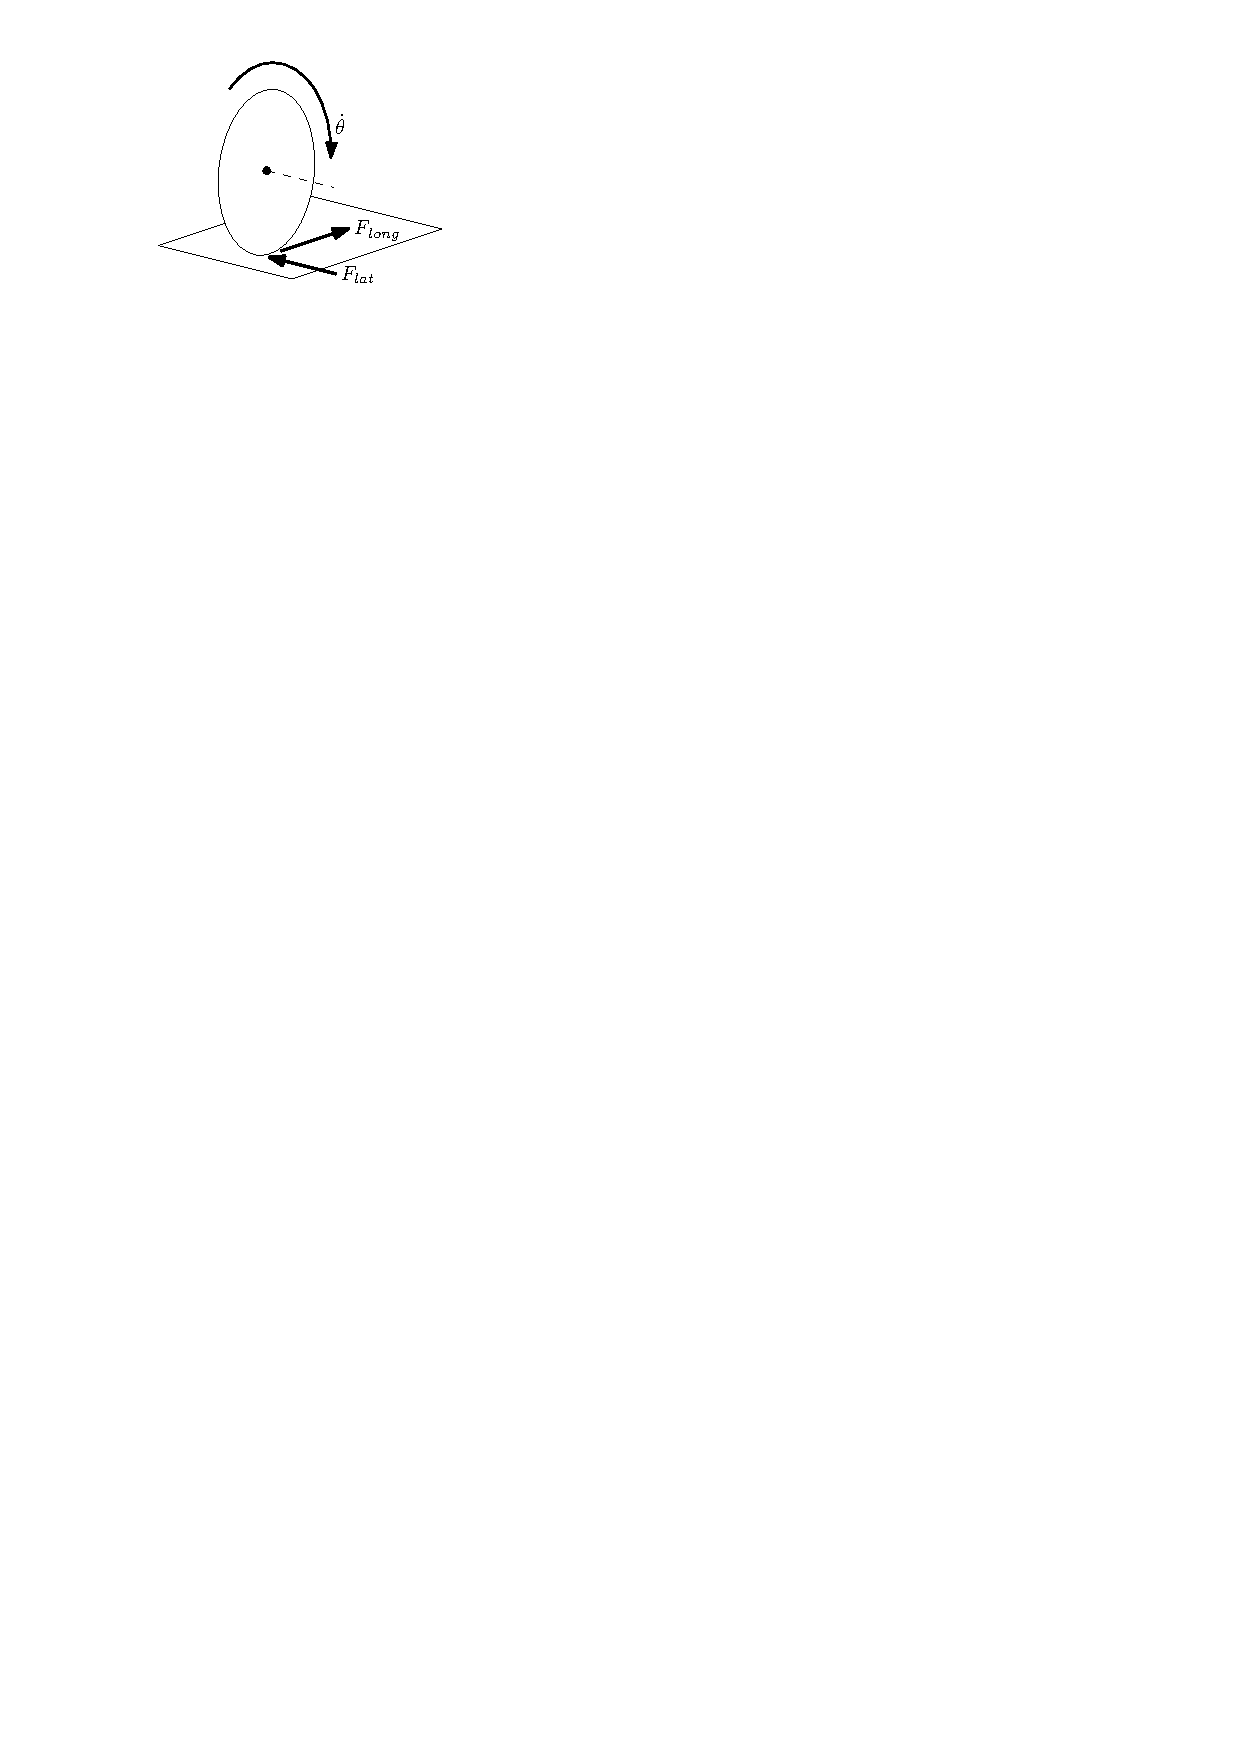
\includegraphics[width=0.7\textwidth]{wheelF.pdf}	%[width=0.9\textwidth]
\caption{Учет сил трения прикладываемых к колесу}
\label{pic:8}
\end{figure}



 


\newpage
\ \\

\section*{Заключение}
\addcontentsline{toc}{section}{Заключение} 

Данный реферат ставил своей целью рассмотреть вывод уравнений движения для мобильных манипуляторов. В работе был представлен краткий обзор области мобильных манипуляторов, для случая колесных платформ были рассмотрены методы математического описания и вывода уравнений движения. 

В частности, для колесных баз дифференциального и всенаправленного типа были рассмотрены кинематические модели и их особенности, основываясь на уравнениях Эйлера-Лагранжа с неопределёнными множителями, соответствующими неголономным связям, в общем виде были получены уравнения движения для мобильных манипуляторов с базой колесного типа.

Особенностью математического описания мобильных манипуляторов является объединение обобщенных координат подвижной базы и манипулятора, а так же учет неголономных связей в виде (\ref{eq:7}) с соответствующими преобразованиями в уравнении Эйлера-Лагранжа. 

Основные сложности при моделировании таких систем в общем случае связанны с избыточностью всей системы и учетом параметров, таких например, как компоненты кинематической модели, обозначающие проскальзывание, которые тяжело или невозможно оценить априорно. 
 

\renewcommand\bibname{\Large{Список использованных источников}}
\begin{thebibliography}{99}
\addcontentsline{toc}{section}{Список использованных источников}
\vspace{-1cm}
{\small
%\hypertarget{Yang}{}
\bibitem{Yang} Yang Lu, Industry 4.0: A survey on technologies, applications and open research issues, In Journal of Industrial Information Integration, Volume 6, 2017, Pages 1-10

\bibitem{Fantini} Fantini, E \& Monica, Francesco \& Occhi, P \& Reggiani, Monica. (2004). Toward a Mobile Manipulator Service Robot for Human Assistance.

\bibitem{Khatib} Oussama Khatib, Mobile manipulation: The robotic assistant, In Robotics and Autonomous Systems, Volume 26, Issues 2–3, 1999, Pages 175-183

\bibitem{Stopp} Towards interactive learning for manufacturing assistants / A. Stopp [et al.] // Robot and
Human Interactive Communication, 2001. Proceedings. 10th IEEE International Workshop
on.  2001. - Pp. 338–342.

\bibitem{Jones} Environmental Hardening of a Mobile-Manipulator System for Nuclear Environments / S. L.
Jones [et al.] // Robotics for Challenging Environments / ed. by L. A. Demsetz, P. R. Klarer. 
1994.  P. 296.

\bibitem{Yang} Yang, Hyunsoo \& Lee, Dongjun. (2014). Dynamics and control of quadrotor with robotic manipulator. Proceedings - IEEE International Conference on Robotics and Automation. 5544-5549

\bibitem{Adamov} Адамов Б. И., Орлов И. В. Управление мобильным манипулятором, работающим в цилиндрической системе координат // Вестник Московского энергетического института. — М., 2012. — No 1. — С. 28—35.

\bibitem{Papad} Papadopoulos E., Poulakakis J. Trajectory planning and control for mobile manipulator systems // The 8th IEEE Mediterranean Conf. on Control \& Automation. — 2000.

\bibitem{Spyros} Spyros G. Tzafestas, In Introduction to Mobile Robot Control, Oxford, 2014, ISBN 9780124170490

\bibitem{Zac} Зацепин М.Ф. Уравнения Лагранжа, Воронца, Чаплыгина в задачах динамики мобильных роботов / М.Ф. Зацепин, Ю.Г. Мартыненко, Д.В. Тиньков. --- М.: Издательство МЭИ, 2005. – 32 с.

\bibitem{Saha} Saha S, Angeles J. Dynamics of Nonholonomic Mechanical Systems Using a Natural Orthogonal Complement. ASME. J. Appl. Mech. 1991;58(1):238-243. 

\bibitem{Korayem} Korayem M., Shafei A., Shafei H. Dynamic modeling of nonholonomic wheeled mobile manipulators with elastic joints using recursive Gibbs---Appell formulation // Scientia Iranica. — 2012. — Vol. 19, no. 4. — Pp. 1092–1104.

\bibitem{Tanner} Tanner, H., \& Kyriakopoulos, K. (2001). Mobile manipulator modeling with Kane's approach. Robotica, 19(6), 675-690.

\bibitem{Hussain} Hussain Z. \& Azlan N. Z. KANE's method for dynamic modeling. Proc. --- IEEE International Conference on Automatic Control and Intelligent Systems. 2016. --- Pp. 174 - 179 

\bibitem{Ariff} F. Ariff, A. Rambely and N. Ghani, "Shoulder’s modeling via Kane’s method: Determination of torques in smash activity", in 5th Kuala Lumpur International Conference on Biomedical Engineering 2011, 2011, pp. 207-209.

\bibitem{Li} Li Z., Ge S. S. Fundamentals in Modeling and Control of Mobile Manipulators. Vol. 49. —
CRC Press, 2013.

\bibitem{Muir} Muir P.F., Neuman C. Kinematic modeling for feedback control of an omnidirectional wheeled mobile robot. In: Proceedings of IEEE international conference on robotics and automation, Raleigh, NC; 1987, p. 1772-8.

\bibitem{Hamid} Hamid Taheri, Bing Qiao and Nurallah Ghaeminezhad. Article: Kinematic Model of a Four Mecanum Wheeled Mobile Robot. International Journal of Computer Applications 113(3):6-9, March 2015.

\bibitem{Borisov} Борисов О.И., Громов В.С., Пыркин А.А., Методы управления робототехническими приложениями. Учебное пособие. — СПб.: Университет ИТМО, 2016. — 108 с.

\bibitem{Buss} Buss S. R. Introduction to inverse kinematics with jacobian transpose, pseudoinverse and damped least squares methods //IEEE Journal of Robotics and Automation. – 2004. – Т. 17. – No. 1-19. – С. 16.

\bibitem{Ben} Ben Kenwright (2012) Inverse Kinematics – Cyclic Coordinate Descent (CCD),
Journal of Graphics Tools, 16:4, 177-217,

\bibitem{Andreas} Andreas Aristidou, Joan Lasenby, FABRIK: A fast, iterative solver for the Inverse Kinematics problem, In Graphical Models, Volume 73, Issue 5, 2011, Pages 243-260, ISSN 1524-0703

}

\end{thebibliography}
%This \hyperlink{Yang}{[1]link} takes you to the same 
%place as \cite{Yang} does.
%\vspace{\fill}
\end{document}
